\chapter{Implementation}

In this chapter we will mention the most important classes of our software and go through their main responsibilities. Here we describe the main three parts of the software - ER/Studio module, PowerDesigner module and the common part used by both of them. The shared module is a general artifact that is designed to be helpful when designing an extractor of metadata from an arbitrary modeling tool that is aimed to be included in Manta Flow. \\

We will go through the implementation from a higher perspective mentioning some classes and their methods from the source code of Metadata Extractor. 
Not every class and method will be described in this chapter, however precise programmer's documentation containing these information comes in a form of JavaDocs.

\section{ER/Studio}

\subsection{File Reverse-Engineering Tool}
\label{subsec:dm1_tool}

We introduced that file format that ER/Studio uses for storing data models consists of a relational databases like CSV tables (see \Cref{subsec:dm1_format}).
In order to be able to deconstruct objects stored in the files, we need to decrypt relations between tables in ER/Studio .DM1 files, as it is not easy to see how structured information is stored in those tables.
The task is to find out what links are leading between tables in the format. Relationships in this type of tabular data storage are done via primary and foreign keys. For this purpose we developed a little reverse engineering tools that should help us to reconstruct complex objects, as aspects of such objects are usually stored in multiple tables. \\

Input for this tool is an arbitrary .DM1 file and output must describe the logical layout. 
We observed the analogy of the file format logic with relational databases, which can be represented understandably by a relational diagram. Thus it would be nice  if output of the tool would be such diagram showing the organization of the .DM1 format.
However to create a diagram directly would be overkill we will use the knowledge that for creation of relational diagrams modeling tools are used.
The tools usually have the ability to transform some procedure defined in SQL into visual representation. 
For example based on the statement CREATE TABLE T modeling tool can draw a box in diagram representing table T. 
SQL surely can define columns of a table and create key constraints on columns as well. 
Modeling tools are able transform a foreign key column in table B that is a primary one in table A into a relationship between the two tables showed graphically in a diagram.

Thus, if we are able to generate a SQL create procedure for each of the tables from the file format and define by the query language primary and foreign keys of the SQL tables, modeling tools would transform such code into a visual representation of the analyzed file format.

To define a SQL create statement for the tables of ER/Studio's file format is straightforward once we parsed a .DM1 file. On the other hand deciding which column of a table is primary, which columns are foreign keys and to primary column of what table they refer to, is a more complicated task.
So we need to take the reverse-engineering process one step further - to be able to infer the keys.
Modeling tools commonly have the ability to reverse-engineer a relational database, however they are not able to tell relations between database tables. If so the knowledge is based on metadata from a database where keys are already defined, while the plain create statement in SQL do not provide any additional information like that.
In this situation we have no better option than to come up with own solution, as we have not found any utility inferring relations between tables solely based on column names or content of database tables.
Output of the reverse engineering tool therefore will be a SQL script containing table and key constraint definitions. 

As the development of the reverse-engineering utility is not the focal point of this work, the utility will not be an out-of-the-box general solution for deducing keys of relational databases, but should provide a basic overview of .DM1 files organization. 
Also it is not going to be a definitive foreign key deducing solution but is primarily concerned with the objects and properties picked by the analysis described above in \Cref{metadata_enumeration}.

In order to create the reverse-engineering utility we must decide what programming language we will write it in. Although there may be scripting languages that would make some operations, like joins on tables easier, we decided to use Java as Metadata Extractor itself is written in it and there is an important module - parser that the column deducing utility and Extractor, require. By developing both in Java it is suffices to write the parser once.\\

Firstly, an analyzed .DM1 file is parsed into a set of \classname{CsvTable}s.

When trying to find out what are columns with key constrained, the idea is to look at the loaded tables from two different views.

The first perspective is to take into account only metadata of a table. This approach is represented by the class \classname{DependencyCreator}. It treats columns that look like keys (eg. those which name ends with "ID", the policy is determined by \methodname{isOnBlacklist} method) as the same across all loaded tables. 
The main method here is \methodname{createDependencies} which pairs potential key columns and tables containing the candidate columns.
The class \classname{RelationFinderByTableDefinitions} allows querying over the structure found by \classname{DependecyCreator} showing what tables are possibly related through a series of joins.
Among others there is a general method \methodname{getDependenciesWithPaths} showing a sequence of joins needed to do in order to put put together records from table A with those from table B.

The second view takes into account data stored in the tables as well. 
When analyzing what are relations between columns, we consider a table as a collection of columns. A \classname{CsvColumn} stores a set of values from all records of its table at position of the column. 
This way we can examine if columns with same names have similar contents.
In contrast when getting records from a table we see it as a collection of \classname{CsvRow}s.
The \classname{RelationFinderByTableContents} class is used for the further search for key columns.

It filters tables that have no content, thus are irrelevant for this approach.
The relation finder class which is analyzing contents of tables has a method for determining if a column can be considered a primary key of a table.  That is true only if a columns contains solely distinct values as a primary key must be completely unique in a table.
The relation finder also has a method finding out if a column can possibly be storing foreign keys. If column A contains foreign keys of primary keys specified in column B, each entry of A must be present in B, thus A must be subset of B.
In .DM1 file format there is a table \classname{Identity Value} that explicitly pairs tables with their primary key columns. Of this information the reverse engineering tool takes advantage as well.
The class also inspects if the primary keys are defined in strict order or if there is some pattern in how primary keys are listed in a .DM1 table.

The classes above allowed us to look from multiple perspectives at metadata and data of tables in the analyzed file format.
To put it all together and to finally generate the desired output in form of a SQL code defining .DM1 tables and their keys out of the analysis done the class \classname{TablesToSQLConverter} is used.
The main method is \methodname{writeMySQLSource} which at the beginning defines SQL create statement for each table from ER/Studio source file. 
Then the phase of creating the key constraints takes place. It operates on candidate columns that satisfy policies in \classname{DepedencyCreator} to be key columns and are present in at least one table so one or more joins can be made using the keys.
There is also space for defining manually the knowledge we gained by inspecting the format using \classname{RelationFinder*} classes by inserting pairs table and its primary key.
At first place primary keys defined from user-defined information are set, then the information stored in \classname{Identity Value} table is used for key definition. Lastly, key inference based on policies a name of a column in context of its table takes place. For example if a table is called tableA\textunderscore id it is very likely it is a primary key if it comes from table called tableA.
If a column is set as a primary key in one table for each of the remaining tables that contains the column with same name, the column is marked as a foreign key.
In the case there are columns that were chosen as candidates for being keys but no constraint was assigned to them in previous steps, in one of the tables which contain such column is marked as a primary and in the rest as a foreign one. That may cause slight inaccuracies in the final result, but the main message should not get lost.

\subsection{Parser}
\label{subsec:dm1_parser}

We already discussed in \Cref{subsec:dm1_format} that the files storing objects we want to recreate from ER/Studio are using format, which is basically a sequence of CSV tables. In order to be able to further process the information saved in the file format, we need to load the contents of those tables into corresponding data structures. That is what parsers are for.

Already existing CSV parsers are made to process a single CSV table per file. There is no unified definition for the comma-separated-value files, but usually they do not allow naming CSV tables as present in .DM1 files.
What is important to say about CSV record is, that each entry is located on a separate line, fields in an entry are separated by a comma, the last record is followed by line break. A field may contain a comma or line break but must be enclosed by double quotes.
If a double quote appears in a field, it must be in the enclosed section and the quote itself must be doubled \cite{RfcCSV}.

The structure we need to parse contains tables consists of a name on a single line, definition of columns and entries. Two tables are separated by a single empty line.

Putting it all together it seemed to be easier to develop our own parser for .DM1 files that processes the files into a set of tables identified by their names.

A single table is represented by an instance of the class \classname{CsvTable} which contains its name, definition of columns, in other words names for each of its properties \classname{CsvColumnDefinition}, and finally records themselves - instances of \classname{CsvColumn} which are contents of a table.

However, the view on a table may vary by usage of the parser. Using the reverse-engineering tool, we inspected what values are stored in a column, examined the domain of values across all records etc. 
On the other hand, if we see a table as records, each record having properties, one property is one column, from this perspective a table is a set of rows.
The second case is needed when reading the contents of a table for the sake of obtaining its records.

Getting a name of a table is an easy job as its just a single textual line. To resolve a record, get the individual fields separated by a comma, correctly is a slightly more challenging task, since the rules described at the beginning of the chapter must be taken into account. 
We designed an automaton that accepts well formed records of our CSV table.

We propose a non-deterministic finite automaton, even though it can be translated to a deterministic one, we consider an NFA to be more clear and descriptive in this situation.
Set of states is $Q = \left\{i, q, e, a, f\right\}$.
Alphabet $\Sigma$ is a set of chars that can appear in a string, since that is what the automaton processes, together with $\lambda$ - an empty string.
I is the initial state.
Transitions are illustrated in the following Figure 5.1.

\begin{figure}[H]
\begin{center}
	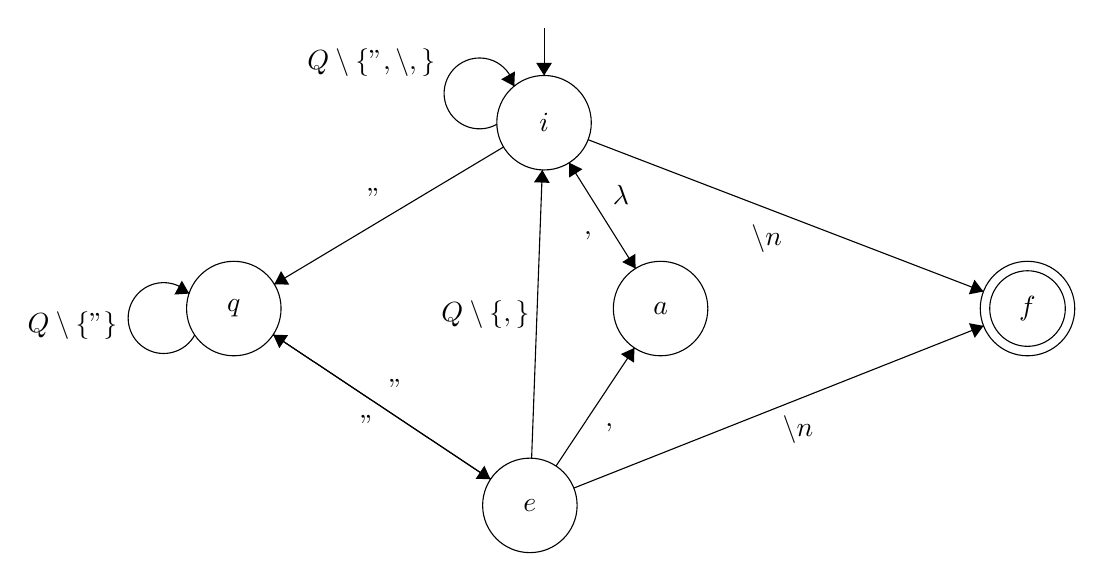
\begin{tikzpicture}[scale=0.2]
	\tikzstyle{every node}+=[inner sep=0pt]
	\draw [black] (40.8,-21.4) circle (3);
	\draw (40.8,-21.4) node {$i$};
	\draw [black] (71.5,-33.2) circle (3);
	\draw (71.5,-33.2) node {$f$};
	\draw [black] (71.5,-33.2) circle (2.4);
	\draw [black] (21.1,-33.2) circle (3);
	\draw (21.1,-33.2) node {$q$};
	\draw [black] (48.2,-33.2) circle (3);
	\draw (48.2,-33.2) node {$a$};
	\draw [black] (39.9,-45.7) circle (3);
	\draw (39.9,-45.7) node {$e$};
	\draw [black] (40.8,-15.4) -- (40.8,-18.4);
	\fill [black] (40.8,-18.4) -- (41.3,-17.6) -- (40.3,-17.6);
	\draw [black] (37.813,-21.495) arc (299.55605:11.55605:2.25);
	\fill [black] (38.91,-19.09) -- (38.95,-18.14) -- (38.08,-18.64);
	\draw (33.93,-17.59) node [left] {$Q\setminus\left\{",\backslash,\right\}$};
	\draw [black] (43.6,-22.48) -- (68.7,-32.12);
	\fill [black] (68.7,-32.12) -- (68.13,-31.37) -- (67.77,-32.3);
	\draw (54.94,-27.83) node [below] {$\backslash n$};
	\draw [black] (38.23,-22.94) -- (23.67,-31.66);
	\fill [black] (23.67,-31.66) -- (24.62,-31.68) -- (24.1,-30.82);
	\draw (30.04,-26.8) node [above] {$"$};
	\draw [black] (18.622,-34.87) arc (-28.28273:-316.28273:2.25);
	\fill [black] (18.27,-32.25) -- (17.8,-31.43) -- (17.33,-32.31);
	\draw (13.73,-34.26) node [left] {$Q\setminus\left\{"\right\}$};
	\draw (39.91,-33.56) node [left] {$Q\setminus\left\{,\right\}$};
	\draw [black] (23.6,-34.86) -- (37.4,-44.04);
	\fill [black] (37.4,-44.04) -- (37.01,-43.18) -- (36.46,-44.01);
	\draw (29.59,-39.95) node [below] {$"$};
	\draw [black] (42.69,-44.6) -- (68.71,-34.3);
	\fill [black] (68.71,-34.3) -- (67.78,-34.13) -- (68.15,-35.06);
	\draw (56.92,-39.97) node [below] {$\backslash n$};
	\draw [black] (41.56,-43.2) -- (46.54,-35.7);
	\fill [black] (46.54,-35.7) -- (45.68,-36.09) -- (46.51,-36.64);
	\draw (44.66,-40.78) node [right] {$,$};
	\draw [black] (37.4,-44.04) -- (23.6,-34.86);
	\fill [black] (23.6,-34.86) -- (23.99,-35.72) -- (24.54,-34.89);
	\draw (31.41,-38.95) node [above] {$"$};
	\draw [black] (40.01,-42.7) -- (40.69,-24.4);
	\fill [black] (40.69,-24.4) -- (40.16,-25.18) -- (41.16,-25.22);
	\draw [black] (46.61,-30.66) -- (42.39,-23.94);
	\fill [black] (42.39,-23.94) -- (42.4,-24.88) -- (43.24,-24.35);
	\fill [black] (46.61,-30.66) -- (46.6,-29.72) -- (45.76,-30.25);
	\draw (45.13,-26.01) node [right] {$\lambda$};
	\draw (43.87,-28.59) node [left] {$,$};
	\end{tikzpicture}
\end{center}
\caption[NFA Accepting a CSV Line]{Non deterministic finite automaton accepting a line of a CSV table in .DM1 file. In the state $a$ and $f$, the end of a CSV field is recognized and accepted.}
\end{figure}

When parsing a CSV record consisting of multiple fields not only we want to determine the end of a CSV entry but to collect the fields as well. That is what the, at first sight redundant, state A expresses. Once the automaton gets to the state $a$, the end of a field in the input is indicated. The boundary of the last field of an entry is, however, recognized in the accepting state $f$.

The parser's interface is a single method \methodname{readFile} taking a file to process and returning pairs of table name and an instance of \classname{CSVTable}.

\subsection{Model}

The purpose of the model component is to provide an access for reading to both a raw structure of a processed source file and a fully loaded hierarchy of objects we reconstructed from a file.

The crucial objects and the important properties of theirs result from the analysis of ER/Studio data models listed in \Cref{metadata_enumeration}. Those are the ones the model is required to capture.

The perspective of a raw file structure loaded to memory is represented by an interface \classname{ErStudioFile} where either all tables from file can be retrieved via \methodname{getAllCsvTables} or a single table by its name using the \methodname{getCsvTable} method.

An ER/Studio solution - a set containing one logical data model and arbitrary number of physical models implements \classname{ErStudioSolution} interface. All the objects contained in the data models stored in such solution can be retrieved using the interface's methods. A solution is defined in a file, the relative name of the file where the solution is an internal one is returned when called \methodname{getFileName}.

Since a .DM1 file is not restricted to storing a single solution, but may reference external models as well, thus there may be objects from multiple solutions saved in a file. If name of the solution's origin file is identical with the name of .DM1 file from which it was loaded, it is an internal file. The overall structure of a file is represented by \classname{ErStudioFileModel} that has a main solution - the internal one and possibly references external solutions.

A base behavior of both logical and physical data models is defined in \classname{DataModel}.
A data model has a name and contains owners. An instance fulfilling \classname{DataModel} interface must have property of type \classname{AbstractionLayer} set to either \methodname{Logical} or \methodname{Physical} just like every object that is contained in a model.

\classname{PhysicalDataModel} has an important addition, that it can tell the database platform the low-level model is designed for. In enum class \classname{Platform} all the database management systems ER/Studio supports are captured with an extra entry for an unknown DBMS.

\classname{Owner} is either \methodname{Logical} or \methodname{Physical} according to what objects it can own and what type of model it may belong to. 
It has name and allows access to the objects owned by it.

The objects that can be mapped to another object implement interface \classname{Mappable<T>} where the type parameter defines what is the kind of the mapped counterpart.

Objects in a data model that can be described further by definition and note while having a name can fit into \classname{DataObject} interface. These can be either \classname{CompositeDataObject} or \classname{SimpleDataObject}.

An interface for the composite ones describes what is expected from a table or an entity.
They have the very same properties that is why a single class is enough to capture their structure. Which of the two it is is decided by \classname{AbstractionLayer}.
The composite one can be mapped to another \classname{CompositeDataObject} and may contain simple objects.

The \classname{SimpleDataObject} class is used to represent columns or attributes. Equivalently, layer of abstraction is crucial to determine whether the object fulfilling the interface can be stored in \classname{PhysicalDataModel} or \classname{LogicalDataModel}. It must be invariant, that the whole subtree of objects, beginning in a data model must have the same abstraction layer defined.

The reason to represent pairs of, at first sight, different concepts of tables-entities and columns-attributes in a single classes is based on how ER/Studio treats them internally. Given that columns and attributes are stored in a single CSV table and the distinction if such object is of one or another type, is made based only on the fact to which data model, physical or logical, it belongs to. The two types have the very same set of possible attributes. This can be applied to composite objects as well. Even data models are treated similarly, only there is an additional attribute related to DBMS type in the case of physical models, while the logical ones do not need such information.
 
\TODO{class diagrams?}
\subsection{Resolver}

The purpose of the resolver unit is to actually create the objects which are form data models which Metadata Extractor obtains from modeling tools. These results of the resolver module, thus are fulfilling the contracts specified by the functionality defined in the model.

Outline of what the resolver module does is that it via \classname{ErStudioFileModelBuilder} creates the whole structure representing an input .DM1 file as instance of \classname{ErStudioFileModel}. It builds an internal solution, then external solutions are created and at the end resolving of mappings that lead across the solution using \classname{ExternalMapper} takes place.

Typically, for each interface, we will create an implementation. In Java it is common to call the classes fulfilling an contract \classname{*Impl} where * is a placeholder for the name of an interface. We stick to this naming convention. 
The \classname{*Impl} classes, in contrast to the interfaces that are used to describe the model component, need to dispose of methods for setting up and adding properties or substructures as the model's reading methods would not be very meaningful otherwise. These classes can be found in the imp package. \\

We defined what is expected from the classes and added the functionality helping to set up the objects, once we gathered required information.
So the last missing piece of puzzle needed to create the objects is how to gather the required information.
The logic taking care of collecting the needed data is hidden in the package builder.
The skeleton of how an instance of \classname{ErStudioSolution} is created is prescribed in the \classname{AbstractDataObjectsBuilder}'s method \methodname{buildErStudioModel} that follows the paradigm of the template method design pattern and defines the steps needed to take in order to construct an instance of \classname{ErStudioSolution} solution, no matter if it is of internal or external type.
The template method enforces a tree of objects in a solution is build from the top down.
The very first is to step is to create a root of such tree - an instance of \classname{ErStudioSolution} that is being build, then \classname{DataModel}s from the solution are loaded, \classname{Owner}s follow, \classname{CompositeObject}s after and finally \classname{SimpleObject}s. 
Child instances are appended to their parents just when created.
The abstract builder contains common methods for construction of objects. Those methods are not dependent on representation, only require a set of properties as input to be able to attach them to resulting objects to make them complete. The groups of properties needed to be collected about each type to proceed the construction are described by interfaces in the package modeledobjectproperties.

The specific way of gathering the information about objects to be reconstructed is tied with details of how the objects are saved in the file format. Concrete builders 	\classname{InternalDataObjectsBuilder} along with \classname{ExternalDataObjectsBuilder} provide implementation to the abstract methods.
In the case of internal solution, information about objects are retrieved from CSV tables, where for each table there is a dedicated and references across the tables are resolved.
On the other hand, in case of external solutions, they are fully represented in a single CSV table that stores XML structures describing these objects. The implementations of the placeholders in \classname{ExternalDataObjectsBuilder} uses a simple SAX XML parser to retrieve the desired data described in modeledobjectproperties.

\classname{InternalDataObjectsBuilder} has one more responsibility and that is to create mappings between \classname{Mappable} objects in a solution with a help of \classname{InternalMapper}. 

The  \classname{InternalMapper} class only has knowledge about the layout of a CSV table containing internal mappings, just like the \classname{ExternalMapper}, that we will need later, has about the definitions of external mappings. However the logic of putting objects to maps-to relation is coded in the \classname{AbstractMapper} class.
It goes through a table which definition fulfills the interface \classname{MappingTable} and links pairs listed in the table by mapping, if their types are equivalent.

\TODO{a class diagram?}

\subsection{Reader}

The reader component puts together the parser module with resolver and produces a data structure by what the model component defined. \\

\classname{ErStudioDm1Reader} crawls through directory with input .DM1 files processing them. Each time the \methodname{read} method is called the parser processes next file from the input folder. Parser's product is handed to resolver resulting in \classname{ErStudioFileModel} that is what \methodname{read} returns.

\subsection{Data Flow Generator}

Having constructed the objects defined in the model unit, Metadata Extractor sends them to Data Flow Generator unit, where the model get transformed into an output graph and connects to Manta Flow to enrich the graph of ER/Studio objects by data lineage.

Before describing the workflow of the generator unit, let us mention its layout.
There is a scenario that executes independent tasks. A task is a routine that has an input and an output. In out case we will use a single task whose input will be a data structure described by the model unit and output a graph with extracted information.

 Namely, \classname{ErStudioDataflowScenario} reads an input file, and executes the task - \classname{ErStudioDataflowTask}. 
 
 The method which tasks must override and gets called is the \methodname{doExecute}. In this particular task it is needed to go through the whole hierarchy of the input data structure - \classname{ErStudioFileModel} unroll solutions - internal as well as external.

A suitable \classname{Connection} corresponding to a physical data model is made of information from a data model and .ini file to be able to pair physical data model objects with those from database dictionaries.

Once assigned the connections to physical models, we can traverse the data models trees, creating nodes using \classname{DatabaseConnector} in the case of physical level, whereas when it comes to logical objects Metadata Extractor takes advantage of \classname{DataModelNodeCreator}.

As the tool creates the mappings symmetrically, the full information is captured on both levels. This way, it is possible to create all the mapping edges by going through all objects from a single level of abstraction, no matter which level though as each mapping edge is contained in both of the levels.
For the sake of simplicity, as there usually is less logical models generally a logical model contains fewer objects than a physical one, data flow generator goes through all the logical objects, creating their node representation and collects the attributes, that have to be linked to a column.
Then physical objects are created as nodes and if the just constructed node has a mapping, MAPS\textunderscore TO edge is set between the mapped nodes.


\section{PowerDesigner}

\subsection{Parser}

The files storing the data model objects we want to reconstruct from PowerDesigner are of XML type.
In the analysis section we already discussed the possibilities when it comes to reading XML files. We concluded that the most suitable approach in our case should be loading the inputs to a DOM tree data structure.
We did not try to reinvent a wheel as there is many DOM parsing services. 
Given that in the ecosystem of Manta software there is an internal artifact made for transforming XML to DOM Metadata Extractor will make use of it.

\subsection{Model}

Let's start describing the main structure the model has to capture generally.
In the case of PowerDesigner a model is saved in a single file. 
Thus \classname{DataModel} has the name of the file where it is stored and its sub objects, then the hierarchy goes like this \classname{Schema} has \classname{CompositeObject}s which contain \classname{SimpleObject}.
This basic skeleton of a tree structure is present in each of the three data models. What more, on logical and conceptual level, as they are represented by an EER diagram, an entity can inherit from another one, thus an interface \classname{Entity} introducing the concept of parent entity will be used by them. Each of actors may have some metadata providing further description and extends the interface of \classname{NamedObject}.
These interfaces are generic and provide the common structure.
For every model type there exists a package, where specific objects' contracts lies. These concrete interfaces on one hand takes over the common concepts. On the other hand may be easily extended if a new functionality, which is data model specific, is identified.

\classname{Mappable} interface is present to be realized on instances of \classname{CompositeObject} or  \classname{SimpleObject}, however a target of a mapping is a globally unique id of an element, not another instance directly. Since by the nature of mappings in PowerDesigner the actual representation may be unreachable yet.

\subsection{Resolver}

The impl package contains the implementational counterpart to the model unit.
Common concepts with no that do not take part in data models in reality and are present to minimize redundancy and provide way to handle similar objects, for example \classname{CompositeObject}, are implemented as abstract classes - their names are prefixed Abstract. The actual objects that are implemented via *Impl classes.

The construction logic of a data model is concentrated in the build sub package.

The API for creating a data structure representing a data model is simply defined by \classname{DataModelBuilder} on what the method \methodname{buildDataModel} may be called and the result is collected from \methodname{getResult} operation.

However, there is a different strategy used for each of the data models based on type it is. So when processing a PowerDesigner file the program must determine the suitable implementation of \classname{DataModelBuilder} accordingly. 
A factory template class \classname{BuilderFactory} is used to determine which implementation - \classname{PhysicalDataModelBuilder} or \classname{LogicalDataModelBuilder} or \classname{ConceptualDataModelBuilder} by the extension of the processed file.

The outline how the builders work is proposed in the \classname{AbstractDataModelBuilder}. Also the functionality independent of type of a specific data model is written here, the way to do it is to look on objects from the perspective of abstract classes providing the general features.

The implementations take an advantage of the fact that forming a tree like structure from an XML format is natural and straightforward, that is why for now we will omit a general point of view on a construction data model that would hide the convenience and context provided straightforwardly by DOM nodes. 
Requests for specific DOM nodes in the builders are done using XPath, which allows querying fully loaded XML trees.

\subsection{Reader}

The reader unit formed by \classname{PowerDesignerXmlComponentReader} reads a directory containing output file of PowerDesigner that are at the same time inputs for Metadata Extractor - .pdm, .ldm or .cdm files and identifies related groups of them. Then proceeds one group after another, in parsing the XML files into a DOM document and passing the DOM trees to resolver that creates a corresponding set of \classname{DataModel} objects using resolver's \classname{DataModelBuilder}, which can be further passed to the data flow generator unit.
 
Input directory containing file to process is the input for \classname{PowerDesignerXmlComponentReader}. The reader recursively discovers the directory and collects the file that will have to be resolved using the \methodname{collectFiles} method. When a data model file is found, its dependencies are checked using a \classname{SAXParser} and a simple handler \classname{TargetSAXHandler} created for the purpose of getting paths to related models from an XML. The found files, however must be in the input directory, so if it is not the case, the reader tries to resolve their paths and check if there is no file with matching sub path within the input directory. If it is a bidirectional edge between the files is created. 
Once all the files from input are collected component creation takes place so the input set is split into smaller logically connected groups.

Then when the main API method of a reader, the \methodname{read} method, is called, it returns one processed component - a set of related reconstructed \classname{DataModel}s. 
That means the reading method is stateful and \methodname{canRead} checks if there are any component left to be returned.

\subsection{Data Flow Generator}

When translating a component of reconstructed data models, a suitable \classname{GraphBuilder} must be chosen based on the layer of abstraction for each data model using \classname{GraphBuilderFactory}.
Then the tree of data model objects is traversed. When dealing with physical data model, \classname{PhysicalGraphBuilder} is used, underlying \classname{DatabaseConnector} searches for the modeled database objects. A suitable \classname{Connection} corresponding to a physical data model is made of information from a data model and .ini file, loading connection details from .dsn and .dcp files is not supported yet.
On the other hand, physical and logical data models use the generic \classname{ModeledGraphBuilder} for creating nodes representing objects brought from data models of greater abstraction.
The generator collects nodes that have mappings by their ids and once all the data models in the processed components are fully built, it means we can resolve the mapping as there are both ends of the MAPS\textunderscore TO type edge we need to create them. Then we simply look at to what ids are objects mapped, obtain an actual representation of these ids put them into the relation by creating the edge.

\section{Extensibility}

For the sake of extracting metadata from modeling tools we developed a unit where a component for a specific tool meets manta flow.
The artifact where the common bridging logic is stored is called manta-dataflow-generator-modeling-common.
Physical data models need to be paired with corresponding connections to DBMS in order to correctly pair the same database objects that appear both in a physical model and in a database dictionary extracted by Manta Flow. This functionality is provided by implementations of interface \classname{DatabaseConnector}. Details about the target database of the low-level data model are kept in \classname{Connection}. The API to database dictionaries created by Manta is provided by \classname{DataflowQueryService}. 
Having collected information of a physical object, either a column or a table, the query service tries to find it in the dictionaries using \methodname{createColumnNode} or \methodname{createTableNode}. 
If the service succeeds, matched node from a dictionary is appended to the output graph, otherwise null is returned from a create method and our tools copes with the situation in such a way, that it creates a node that has no backing in a live database, marking the node's attribute source type to MODEL to make clear in the output, that it is an artificial node based only on a physical data model. It can be from two reasons - the database object does not exists or we provided inaccurate/incomplete data to identify it.

So the first general requirement for a general extractor from data modeling tools is to be able to organize extracted metadata in such a way that \classname{DatabaseConnector} may be called and ideally match the modeled objects with the extracted ones.
This is a very important step as this pairing is the prerequisite for business data lineage creation. If the physical modeled object do not match the ones from database that take part in data lineage, there is no flow to be propagate to higher levels of abstraction via maps to edges and the result of interpolation will be an empty set of edges.

Secondly, we have defined a common way of creating nodes representing objects extracted from data models of higher abstraction than the physical ones - conceptual and logical.
We define a set of methods where each is responsible for creation of node representation of a type of object that may appear in the data models. Most commonly a modeling tool will support only subset of the types the node creator is able to construct. However that is not a problem as the hierarchy is not strict and it can be built to be compliant with concepts of a specific modeling tool. 
For example it is not necessary to build an attribute under an entity node if a modeling tool does not allow such concept, just like an owner node is not necessary as there is no strict rule if the tools should support it or not.

We have discussed the modeled objects on conceptual and logical level are described by ER or EER diagrams. 
The important fact is that the possible kinds of objects will be the same in both models, that is why a single interface \classname{DataModelNodeCreator} for high-level node creation may be used.
However it must be implemented by two different classes \classname{LogicalDataModelNodeCreatorImpl} and \classname{ConceptualDataModelNodeCreatorImpl}, so details about node's type can be specified, therefore the nodes will not mix between the layers.
\classname{Resource} differentiates technologies, in our case it makes sure objects extracted from modeling tools are aggregated by what specific tool is their origin.

To attach metadata about a node, such as its definition or a comment, object that is being transformed into node representation has to implement interface \classname{NodeMetadata}.
The contract forces the implementers to expose the metadata to be attached to node representing them in the output in form of strings. 
More precisely, the objects have to fill a \classname{Map<String, String>} data structure where a key is the name of a property. 
These metadata are shown when presenting the output graph and further describe the extracted objects. \\ 

Basically, the outline when implementing a metadata extraction from a different modeling tool is the following:

\begin{enumerate}
	\item Define the crucial data model objects, relations between them, hierarchy and properties interesting enough to be captured in data lineage by read-only interfaces. That is model component. 
	The objects that will be represented as standalone nodes in data lineage visualization at the end have to implement \classname{NodeMetadata} interface.
	\item Depending where from the data models are obtained, this phase generally retrieves data models from a storage. It may be by calling a web API to get data mode objects from a server, retrieving them from a database, or like in the case of Metadata Extractor, by parsing a file.
	\item Resolving takes place once some representation of data models was reached. This stage transforms the acquired object into objects conforming aspects described by the model module.
	\item Data flow is generated from the output of the resolver. This module translates data structures describing modeled objects to graph nodes. 
	Database objects from physical data models are expected match the ones in database dictionaries of Manta that were extracted directly from databases. 
	The communication with Manta is done via \classname{DatabaseConnector} and \classname{Connection} that is assigned to a physical model.
	Logical and physical modeled objects are transformed to node representation using corresponding implementation of \classname{DataModelNodeCreator} - logical and physical respectively.
	Once the nodes are created out of the extracted objects, resolving of mappings between the layers takes place.
	Linking correctly physical nodes, that were paired with the ones from database dictionary, with higher level nodes is crucial to bring business lineage. 
	However there is no strict skeleton for this process as the approaches to how modeling tool realizes mapping across data models may be substantially different, as we have seen in case of PowerDesigner and ER/Studio.
\end{enumerate} 

\section{Technologies}

The quality of programmer's toolbox may have a huge influence on his productivity when developing a more complex piece of software.

\begin{itemize}
	\item Java 8 \\
	To be able to integrate Metadata Extractor into the ecosystem of Manta Flow the best solution is to use Java as the APIs of the data lineage software are written in this programming language.
	\item Maven \\ 
	For dependency management, the most usual tool when programming in Java is used - Maven. In order to build the program, all the Manta Flow artifacts which Metadata Extractor depends on must be obtained successfully. However those artifacts are reachable only within Manta's private network.
	\item Spring \\
	For program configuration, inversion of control via Spring's XML files is used. Along with .properties, where variables used in the spring files may be (re)defined.
	\item JUnit 4 \\ 
	The standard for unit testing Java programs is the JUnit framework we use.
\end{itemize}

\section{Testing}

Automated unit tests validating the crucial parts of the implementation are a huge help to determine correctness of Metadata Extractor's logic.

\subsubsection{ER/Studio Parser}

The correctness of parsing process is checked by class \classname{ErStudioFileFormatParserTest} which is controlling how many CSV tables from a parsed .DM1 files was obtained. Given that the format consists of a constant number of tables if the count is mismatching it indicates a flaw in detecting borders of tables.
Also every CSVs should be valid in the way that each row in a table must have the same number of fields. If it has not, we assume there is problem on our side and parser does not pass the tests.

\subsubsection{Reader \& Resolver}

Testing of the output of the reader module shows tells a lot about the resolver's correctness, since the logic of reader is actually provided by this module. 
From the nature of reader, that it connects resolver and parser, these tests rely on the fact that resolver works correctly and we assume this is true as far as the parser module tests are passing.
The goal of the reader tests is to find out whether all objects from data models were successfully loaded into data structures described by the model module.
In case of ER/Studio the testing compares expected statistics about data models such as number of physical models in a solution, entity count of logical model etc. with the amount of objects that were loaded actually by reader.
Secondly, some specific objects from hierarchy of a data model that is on input are picked and checked if they were loaded accordingly. Tests check metadata of those objects and mappings with another objects as well. \\ 

PowerDesigner must create components correctly, so is present a test for checking if number of components is correct.
The main reader test consists of reading file by file, thus size of a component is one every time (the components creation correctness is ensured the previous test).
The expected values and objects are loaded from JSON sources file where they are stored in a deserialized form.

\subsubsection{Data Flow Generator}

In data flow generator, we are interested if objects loaded by reader are transformed into nodes as expected.
The skeleton is similar for both modeling tools. \\

\classname{*GraphBuilderTest} classes are testing independently drawing of each of the layers. The graph created by the \classname{*GraphBuilder} classes can be saved as a .txt file describing the graph. 
For each test we have an expected output of how a correct output graph should look like. The two files are compared, if they are same the behavior of the output building process is correct.

The previous test checked the representation of the layers independently, in \classname{*DataflowTaskTest} all layers from a solution, or from a component when talking about PowerDesigner, are constructed with mapping edges leading between them. Outputting graph is also serialized to a textual file. Next, mapping edges are filtered from the file and compared with expected set of maps\textunderscore to edges. 



